% Options for packages loaded elsewhere
% Options for packages loaded elsewhere
\PassOptionsToPackage{unicode}{hyperref}
\PassOptionsToPackage{hyphens}{url}
\PassOptionsToPackage{dvipsnames,svgnames,x11names}{xcolor}
%
\documentclass[
  letterpaper,
  DIV=11,
  numbers=noendperiod]{scrartcl}
\usepackage{xcolor}
\usepackage{amsmath,amssymb}
\setcounter{secnumdepth}{-\maxdimen} % remove section numbering
\usepackage{iftex}
\ifPDFTeX
  \usepackage[T1]{fontenc}
  \usepackage[utf8]{inputenc}
  \usepackage{textcomp} % provide euro and other symbols
\else % if luatex or xetex
  \usepackage{unicode-math} % this also loads fontspec
  \defaultfontfeatures{Scale=MatchLowercase}
  \defaultfontfeatures[\rmfamily]{Ligatures=TeX,Scale=1}
\fi
\usepackage{lmodern}
\ifPDFTeX\else
  % xetex/luatex font selection
\fi
% Use upquote if available, for straight quotes in verbatim environments
\IfFileExists{upquote.sty}{\usepackage{upquote}}{}
\IfFileExists{microtype.sty}{% use microtype if available
  \usepackage[]{microtype}
  \UseMicrotypeSet[protrusion]{basicmath} % disable protrusion for tt fonts
}{}
\makeatletter
\@ifundefined{KOMAClassName}{% if non-KOMA class
  \IfFileExists{parskip.sty}{%
    \usepackage{parskip}
  }{% else
    \setlength{\parindent}{0pt}
    \setlength{\parskip}{6pt plus 2pt minus 1pt}}
}{% if KOMA class
  \KOMAoptions{parskip=half}}
\makeatother
% Make \paragraph and \subparagraph free-standing
\makeatletter
\ifx\paragraph\undefined\else
  \let\oldparagraph\paragraph
  \renewcommand{\paragraph}{
    \@ifstar
      \xxxParagraphStar
      \xxxParagraphNoStar
  }
  \newcommand{\xxxParagraphStar}[1]{\oldparagraph*{#1}\mbox{}}
  \newcommand{\xxxParagraphNoStar}[1]{\oldparagraph{#1}\mbox{}}
\fi
\ifx\subparagraph\undefined\else
  \let\oldsubparagraph\subparagraph
  \renewcommand{\subparagraph}{
    \@ifstar
      \xxxSubParagraphStar
      \xxxSubParagraphNoStar
  }
  \newcommand{\xxxSubParagraphStar}[1]{\oldsubparagraph*{#1}\mbox{}}
  \newcommand{\xxxSubParagraphNoStar}[1]{\oldsubparagraph{#1}\mbox{}}
\fi
\makeatother

\usepackage{color}
\usepackage{fancyvrb}
\newcommand{\VerbBar}{|}
\newcommand{\VERB}{\Verb[commandchars=\\\{\}]}
\DefineVerbatimEnvironment{Highlighting}{Verbatim}{commandchars=\\\{\}}
% Add ',fontsize=\small' for more characters per line
\usepackage{framed}
\definecolor{shadecolor}{RGB}{241,243,245}
\newenvironment{Shaded}{\begin{snugshade}}{\end{snugshade}}
\newcommand{\AlertTok}[1]{\textcolor[rgb]{0.68,0.00,0.00}{#1}}
\newcommand{\AnnotationTok}[1]{\textcolor[rgb]{0.37,0.37,0.37}{#1}}
\newcommand{\AttributeTok}[1]{\textcolor[rgb]{0.40,0.45,0.13}{#1}}
\newcommand{\BaseNTok}[1]{\textcolor[rgb]{0.68,0.00,0.00}{#1}}
\newcommand{\BuiltInTok}[1]{\textcolor[rgb]{0.00,0.23,0.31}{#1}}
\newcommand{\CharTok}[1]{\textcolor[rgb]{0.13,0.47,0.30}{#1}}
\newcommand{\CommentTok}[1]{\textcolor[rgb]{0.37,0.37,0.37}{#1}}
\newcommand{\CommentVarTok}[1]{\textcolor[rgb]{0.37,0.37,0.37}{\textit{#1}}}
\newcommand{\ConstantTok}[1]{\textcolor[rgb]{0.56,0.35,0.01}{#1}}
\newcommand{\ControlFlowTok}[1]{\textcolor[rgb]{0.00,0.23,0.31}{\textbf{#1}}}
\newcommand{\DataTypeTok}[1]{\textcolor[rgb]{0.68,0.00,0.00}{#1}}
\newcommand{\DecValTok}[1]{\textcolor[rgb]{0.68,0.00,0.00}{#1}}
\newcommand{\DocumentationTok}[1]{\textcolor[rgb]{0.37,0.37,0.37}{\textit{#1}}}
\newcommand{\ErrorTok}[1]{\textcolor[rgb]{0.68,0.00,0.00}{#1}}
\newcommand{\ExtensionTok}[1]{\textcolor[rgb]{0.00,0.23,0.31}{#1}}
\newcommand{\FloatTok}[1]{\textcolor[rgb]{0.68,0.00,0.00}{#1}}
\newcommand{\FunctionTok}[1]{\textcolor[rgb]{0.28,0.35,0.67}{#1}}
\newcommand{\ImportTok}[1]{\textcolor[rgb]{0.00,0.46,0.62}{#1}}
\newcommand{\InformationTok}[1]{\textcolor[rgb]{0.37,0.37,0.37}{#1}}
\newcommand{\KeywordTok}[1]{\textcolor[rgb]{0.00,0.23,0.31}{\textbf{#1}}}
\newcommand{\NormalTok}[1]{\textcolor[rgb]{0.00,0.23,0.31}{#1}}
\newcommand{\OperatorTok}[1]{\textcolor[rgb]{0.37,0.37,0.37}{#1}}
\newcommand{\OtherTok}[1]{\textcolor[rgb]{0.00,0.23,0.31}{#1}}
\newcommand{\PreprocessorTok}[1]{\textcolor[rgb]{0.68,0.00,0.00}{#1}}
\newcommand{\RegionMarkerTok}[1]{\textcolor[rgb]{0.00,0.23,0.31}{#1}}
\newcommand{\SpecialCharTok}[1]{\textcolor[rgb]{0.37,0.37,0.37}{#1}}
\newcommand{\SpecialStringTok}[1]{\textcolor[rgb]{0.13,0.47,0.30}{#1}}
\newcommand{\StringTok}[1]{\textcolor[rgb]{0.13,0.47,0.30}{#1}}
\newcommand{\VariableTok}[1]{\textcolor[rgb]{0.07,0.07,0.07}{#1}}
\newcommand{\VerbatimStringTok}[1]{\textcolor[rgb]{0.13,0.47,0.30}{#1}}
\newcommand{\WarningTok}[1]{\textcolor[rgb]{0.37,0.37,0.37}{\textit{#1}}}

\usepackage{longtable,booktabs,array}
\usepackage{calc} % for calculating minipage widths
% Correct order of tables after \paragraph or \subparagraph
\usepackage{etoolbox}
\makeatletter
\patchcmd\longtable{\par}{\if@noskipsec\mbox{}\fi\par}{}{}
\makeatother
% Allow footnotes in longtable head/foot
\IfFileExists{footnotehyper.sty}{\usepackage{footnotehyper}}{\usepackage{footnote}}
\makesavenoteenv{longtable}
\usepackage{graphicx}
\makeatletter
\newsavebox\pandoc@box
\newcommand*\pandocbounded[1]{% scales image to fit in text height/width
  \sbox\pandoc@box{#1}%
  \Gscale@div\@tempa{\textheight}{\dimexpr\ht\pandoc@box+\dp\pandoc@box\relax}%
  \Gscale@div\@tempb{\linewidth}{\wd\pandoc@box}%
  \ifdim\@tempb\p@<\@tempa\p@\let\@tempa\@tempb\fi% select the smaller of both
  \ifdim\@tempa\p@<\p@\scalebox{\@tempa}{\usebox\pandoc@box}%
  \else\usebox{\pandoc@box}%
  \fi%
}
% Set default figure placement to htbp
\def\fps@figure{htbp}
\makeatother





\setlength{\emergencystretch}{3em} % prevent overfull lines

\providecommand{\tightlist}{%
  \setlength{\itemsep}{0pt}\setlength{\parskip}{0pt}}



 


\usepackage{booktabs}
\usepackage{longtable}
\usepackage{array}
\usepackage{multirow}
\usepackage{wrapfig}
\usepackage{float}
\usepackage{colortbl}
\usepackage{pdflscape}
\usepackage{tabu}
\usepackage{threeparttable}
\usepackage{threeparttablex}
\usepackage[normalem]{ulem}
\usepackage{makecell}
\usepackage{xcolor}
\KOMAoption{captions}{tableheading}
\makeatletter
\@ifpackageloaded{caption}{}{\usepackage{caption}}
\AtBeginDocument{%
\ifdefined\contentsname
  \renewcommand*\contentsname{Table of contents}
\else
  \newcommand\contentsname{Table of contents}
\fi
\ifdefined\listfigurename
  \renewcommand*\listfigurename{List of Figures}
\else
  \newcommand\listfigurename{List of Figures}
\fi
\ifdefined\listtablename
  \renewcommand*\listtablename{List of Tables}
\else
  \newcommand\listtablename{List of Tables}
\fi
\ifdefined\figurename
  \renewcommand*\figurename{Figure}
\else
  \newcommand\figurename{Figure}
\fi
\ifdefined\tablename
  \renewcommand*\tablename{Table}
\else
  \newcommand\tablename{Table}
\fi
}
\@ifpackageloaded{float}{}{\usepackage{float}}
\floatstyle{ruled}
\@ifundefined{c@chapter}{\newfloat{codelisting}{h}{lop}}{\newfloat{codelisting}{h}{lop}[chapter]}
\floatname{codelisting}{Listing}
\newcommand*\listoflistings{\listof{codelisting}{List of Listings}}
\makeatother
\makeatletter
\makeatother
\makeatletter
\@ifpackageloaded{caption}{}{\usepackage{caption}}
\@ifpackageloaded{subcaption}{}{\usepackage{subcaption}}
\makeatother
\usepackage{bookmark}
\IfFileExists{xurl.sty}{\usepackage{xurl}}{} % add URL line breaks if available
\urlstyle{same}
\hypersetup{
  pdftitle={Entrega},
  pdfauthor={Romero Vázquez Ángel Eladio; Solano Tavera Andrea},
  colorlinks=true,
  linkcolor={blue},
  filecolor={Maroon},
  citecolor={Blue},
  urlcolor={Blue},
  pdfcreator={LaTeX via pandoc}}


\title{Entrega}
\author{Romero Vázquez Ángel Eladio \and Solano Tavera Andrea}
\date{}
\begin{document}
\maketitle


\#\#\#Introducción En este trabajo se analiza el comportamiento de la
mortalidad en el estado de Campeche durante los años 2010, 2019 y 2021.
Estos años permiten comparar tres momentos importantes: 2010 como punto
inicial de referencia censal, 2019 como año previo a la pandemia por
COVID-19 y 2021 como un año afectado por sus efectos en la mortalidad.
Campeche es una entidad ubicada en el sureste de México, dentro de la
península de Yucatán. Se caracteriza por tener una población
relativamente pequeña y una baja densidad poblacional, lo que puede
influir en la distribución de los servicios de salud y en el acceso
oportuno a la atención médica. En 2010, el estado tenía 822,441
habitantes, mientras que para 2020 alcanzó 928,363 habitantes, lo que
muestra un crecimiento moderado de la población. Otro aspecto importante
es el cambio en la estructura por edad. En 2010, Campeche tenía una edad
mediana de 25 años, mientras que en 2020 aumentó a 29 años, lo cual
indica un avance gradual hacia el envejecimiento demográfico. Este dato
es relevante porque una población con mayor proporción de adultos
mayores tiende a presentar niveles más altos de mortalidad. Además, el
año 2021 debe interpretarse con cuidado, ya que la mortalidad estuvo
influida por la pandemia por COVID-19. Por ello, al comparar 2019 con
2021, se puede observar no solo el comportamiento habitual de la
mortalidad, sino también el efecto de un evento sanitario
extraordinario. En conjunto, estos elementos permiten contextualizar los
resultados del análisis, considerando que la mortalidad en Campeche
puede estar relacionada tanto con su estructura poblacional como con
factores territoriales y de acceso a servicios de salud. En particular,
se considerarán elementos como la estructura por edad, la distribución
por sexo, el crecimiento poblacional y la densidad demográfica, ya que
estos factores sirven como base para interpretar posteriormente las
tasas de mortalidad y sus posibles diferencias dentro del estado.
\#\#Librerias y carga de data

\begin{verbatim}
[1] "00_Pob_Mitad_1950_2070.csv"     "Data entrega final"            
[3] "Mortaliad_y_proyección.csv"     "Mortaliad_y_proyección.xlsx"   
[5] "mortalidad_2010_2019_2021.csv"  "mortalidad_2010_2019_2021.xlsx"
\end{verbatim}

\subsubsection{Creación de una primer tabla de
mortalidad}\label{creaciuxf3n-de-una-primer-tabla-de-mortalidad}

\begin{verbatim}
[1] "00_Pob_Mitad_1950_2070.csv"     "Data entrega final"            
[3] "Mortaliad_y_proyección.csv"     "Mortaliad_y_proyección.xlsx"   
[5] "mortalidad_2010_2019_2021.csv"  "mortalidad_2010_2019_2021.xlsx"
\end{verbatim}

\begin{verbatim}
[1] "Edad"   "AÑO"    "Hombre" "Mujer" 
\end{verbatim}

\subsubsection{Obtenemos las tablas de vida de cada
año}\label{obtenemos-las-tablas-de-vida-de-cada-auxf1o}

\section{Tabla de vida obtenida con los datos de
2010}\label{tabla-de-vida-obtenida-con-los-datos-de-2010}

\begin{Shaded}
\begin{Highlighting}[]
\CommentTok{\#Tabla de vida 2010}
\NormalTok{lt2010 }\OtherTok{\textless{}{-}}\NormalTok{ lt1 }\SpecialCharTok{\%\textgreater{}\%}
  \FunctionTok{filter}\NormalTok{(AÑO }\SpecialCharTok{==} \DecValTok{2010}\NormalTok{) }\SpecialCharTok{\%\textgreater{}\%}
    \FunctionTok{select}\NormalTok{(}\SpecialCharTok{{-}}\NormalTok{AÑO)}
\end{Highlighting}
\end{Shaded}

\#Tabla de vida obtenido con los datos de 2019

\begin{Shaded}
\begin{Highlighting}[]
\CommentTok{\#Tabla de vida 2019}
\NormalTok{lt2019 }\OtherTok{\textless{}{-}}\NormalTok{ lt1 }\SpecialCharTok{\%\textgreater{}\%}
  \FunctionTok{filter}\NormalTok{(AÑO }\SpecialCharTok{==} \DecValTok{2019}\NormalTok{) }\SpecialCharTok{\%\textgreater{}\%}
    \FunctionTok{select}\NormalTok{(}\SpecialCharTok{{-}}\NormalTok{AÑO)}
\FunctionTok{kable}\NormalTok{(lt2019, }
      \AttributeTok{caption =} \StringTok{"Tabla de vida 2019"}\NormalTok{, }
      \AttributeTok{align =} \StringTok{"c"}\NormalTok{)}
\end{Highlighting}
\end{Shaded}

\begin{longtable}[]{@{}
  >{\centering\arraybackslash}p{(\linewidth - 54\tabcolsep) * \real{0.0156}}
  >{\centering\arraybackslash}p{(\linewidth - 54\tabcolsep) * \real{0.0117}}
  >{\centering\arraybackslash}p{(\linewidth - 54\tabcolsep) * \real{0.0233}}
  >{\centering\arraybackslash}p{(\linewidth - 54\tabcolsep) * \real{0.0233}}
  >{\centering\arraybackslash}p{(\linewidth - 54\tabcolsep) * \real{0.0195}}
  >{\centering\arraybackslash}p{(\linewidth - 54\tabcolsep) * \real{0.0195}}
  >{\centering\arraybackslash}p{(\linewidth - 54\tabcolsep) * \real{0.0195}}
  >{\centering\arraybackslash}p{(\linewidth - 54\tabcolsep) * \real{0.0272}}
  >{\centering\arraybackslash}p{(\linewidth - 54\tabcolsep) * \real{0.0428}}
  >{\centering\arraybackslash}p{(\linewidth - 54\tabcolsep) * \real{0.0428}}
  >{\centering\arraybackslash}p{(\linewidth - 54\tabcolsep) * \real{0.0428}}
  >{\centering\arraybackslash}p{(\linewidth - 54\tabcolsep) * \real{0.0428}}
  >{\centering\arraybackslash}p{(\linewidth - 54\tabcolsep) * \real{0.0428}}
  >{\centering\arraybackslash}p{(\linewidth - 54\tabcolsep) * \real{0.0428}}
  >{\centering\arraybackslash}p{(\linewidth - 54\tabcolsep) * \real{0.0428}}
  >{\centering\arraybackslash}p{(\linewidth - 54\tabcolsep) * \real{0.0428}}
  >{\centering\arraybackslash}p{(\linewidth - 54\tabcolsep) * \real{0.0428}}
  >{\centering\arraybackslash}p{(\linewidth - 54\tabcolsep) * \real{0.0428}}
  >{\centering\arraybackslash}p{(\linewidth - 54\tabcolsep) * \real{0.0389}}
  >{\centering\arraybackslash}p{(\linewidth - 54\tabcolsep) * \real{0.0428}}
  >{\centering\arraybackslash}p{(\linewidth - 54\tabcolsep) * \real{0.0428}}
  >{\centering\arraybackslash}p{(\linewidth - 54\tabcolsep) * \real{0.0389}}
  >{\centering\arraybackslash}p{(\linewidth - 54\tabcolsep) * \real{0.0428}}
  >{\centering\arraybackslash}p{(\linewidth - 54\tabcolsep) * \real{0.0389}}
  >{\centering\arraybackslash}p{(\linewidth - 54\tabcolsep) * \real{0.0389}}
  >{\centering\arraybackslash}p{(\linewidth - 54\tabcolsep) * \real{0.0428}}
  >{\centering\arraybackslash}p{(\linewidth - 54\tabcolsep) * \real{0.0428}}
  >{\centering\arraybackslash}p{(\linewidth - 54\tabcolsep) * \real{0.0428}}@{}}
\caption{Tabla de vida 2019}\tabularnewline
\toprule\noalign{}
\begin{minipage}[b]{\linewidth}\centering
x
\end{minipage} & \begin{minipage}[b]{\linewidth}\centering
n
\end{minipage} & \begin{minipage}[b]{\linewidth}\centering
Hlx
\end{minipage} & \begin{minipage}[b]{\linewidth}\centering
Mlx
\end{minipage} & \begin{minipage}[b]{\linewidth}\centering
HDx
\end{minipage} & \begin{minipage}[b]{\linewidth}\centering
MDx
\end{minipage} & \begin{minipage}[b]{\linewidth}\centering
Dx
\end{minipage} & \begin{minipage}[b]{\linewidth}\centering
lx
\end{minipage} & \begin{minipage}[b]{\linewidth}\centering
q\_x
\end{minipage} & \begin{minipage}[b]{\linewidth}\centering
qx\_h
\end{minipage} & \begin{minipage}[b]{\linewidth}\centering
qx\_m
\end{minipage} & \begin{minipage}[b]{\linewidth}\centering
p\_x
\end{minipage} & \begin{minipage}[b]{\linewidth}\centering
px\_h
\end{minipage} & \begin{minipage}[b]{\linewidth}\centering
q0\_h\_anio
\end{minipage} & \begin{minipage}[b]{\linewidth}\centering
q0\_m\_anio
\end{minipage} & \begin{minipage}[b]{\linewidth}\centering
q0\_anio
\end{minipage} & \begin{minipage}[b]{\linewidth}\centering
ax\_h
\end{minipage} & \begin{minipage}[b]{\linewidth}\centering
ax\_m
\end{minipage} & \begin{minipage}[b]{\linewidth}\centering
ax\_gen
\end{minipage} & \begin{minipage}[b]{\linewidth}\centering
HLx
\end{minipage} & \begin{minipage}[b]{\linewidth}\centering
MLx
\end{minipage} & \begin{minipage}[b]{\linewidth}\centering
Lx
\end{minipage} & \begin{minipage}[b]{\linewidth}\centering
Tx
\end{minipage} & \begin{minipage}[b]{\linewidth}\centering
HTx
\end{minipage} & \begin{minipage}[b]{\linewidth}\centering
MTx
\end{minipage} & \begin{minipage}[b]{\linewidth}\centering
ex
\end{minipage} & \begin{minipage}[b]{\linewidth}\centering
ex\_h
\end{minipage} & \begin{minipage}[b]{\linewidth}\centering
ex\_m
\end{minipage} \\
\midrule\noalign{}
\endfirsthead
\toprule\noalign{}
\begin{minipage}[b]{\linewidth}\centering
x
\end{minipage} & \begin{minipage}[b]{\linewidth}\centering
n
\end{minipage} & \begin{minipage}[b]{\linewidth}\centering
Hlx
\end{minipage} & \begin{minipage}[b]{\linewidth}\centering
Mlx
\end{minipage} & \begin{minipage}[b]{\linewidth}\centering
HDx
\end{minipage} & \begin{minipage}[b]{\linewidth}\centering
MDx
\end{minipage} & \begin{minipage}[b]{\linewidth}\centering
Dx
\end{minipage} & \begin{minipage}[b]{\linewidth}\centering
lx
\end{minipage} & \begin{minipage}[b]{\linewidth}\centering
q\_x
\end{minipage} & \begin{minipage}[b]{\linewidth}\centering
qx\_h
\end{minipage} & \begin{minipage}[b]{\linewidth}\centering
qx\_m
\end{minipage} & \begin{minipage}[b]{\linewidth}\centering
p\_x
\end{minipage} & \begin{minipage}[b]{\linewidth}\centering
px\_h
\end{minipage} & \begin{minipage}[b]{\linewidth}\centering
q0\_h\_anio
\end{minipage} & \begin{minipage}[b]{\linewidth}\centering
q0\_m\_anio
\end{minipage} & \begin{minipage}[b]{\linewidth}\centering
q0\_anio
\end{minipage} & \begin{minipage}[b]{\linewidth}\centering
ax\_h
\end{minipage} & \begin{minipage}[b]{\linewidth}\centering
ax\_m
\end{minipage} & \begin{minipage}[b]{\linewidth}\centering
ax\_gen
\end{minipage} & \begin{minipage}[b]{\linewidth}\centering
HLx
\end{minipage} & \begin{minipage}[b]{\linewidth}\centering
MLx
\end{minipage} & \begin{minipage}[b]{\linewidth}\centering
Lx
\end{minipage} & \begin{minipage}[b]{\linewidth}\centering
Tx
\end{minipage} & \begin{minipage}[b]{\linewidth}\centering
HTx
\end{minipage} & \begin{minipage}[b]{\linewidth}\centering
MTx
\end{minipage} & \begin{minipage}[b]{\linewidth}\centering
ex
\end{minipage} & \begin{minipage}[b]{\linewidth}\centering
ex\_h
\end{minipage} & \begin{minipage}[b]{\linewidth}\centering
ex\_m
\end{minipage} \\
\midrule\noalign{}
\endhead
\bottomrule\noalign{}
\endlastfoot
0 & 1 & 7787 & 7509 & 103 & 87 & 190 & 15296 & 0.0124215 & 0.0132272 &
0.0115861 & 0.9875785 & 0.9884139 & 0.0132272 & 0.0115861 & 0.0124215 &
0.0805281 & 0.0824411 & 0.078212 & 7795.294 & 7516.172 & 15310.86 &
1271032.6 & 635245.7 & 635785.8 & 83.095750 & 81.577713 & 84.669830 \\
1 & 4 & 7684 & 7422 & 12 & 16 & 28 & 15106 & 0.0018536 & 0.0015617 &
0.0021558 & 0.9981464 & 0.9978442 & 0.0132272 & 0.0115861 & 0.0124215 &
1.6131465 & 1.5052074 & 1.615574 & 30755.358 & 29712.083 & 60469.24 &
1255721.7 & 627450.4 & 628269.6 & 83.127349 & 81.656736 & 84.649634 \\
5 & 5 & 7672 & 7406 & 14 & 9 & 23 & 15078 & 0.0015254 & 0.0018248 &
0.0012152 & 0.9984746 & 0.9987848 & 0.0132272 & 0.0115861 & 0.0124215 &
2.5000000 & 2.5000000 & 2.500000 & 38395.000 & 37052.500 & 75447.50 &
1195252.5 & 596695.0 & 598557.5 & 79.271289 & 77.775678 & 80.820618 \\
10 & 5 & 7658 & 7397 & 11 & 10 & 21 & 15055 & 0.0013949 & 0.0014364 &
0.0013519 & 0.9986051 & 0.9986481 & 0.0132272 & 0.0115861 & 0.0124215 &
2.5000000 & 2.5000000 & 2.500000 & 38317.500 & 37010.000 & 75327.50 &
1119805.0 & 558300.0 & 561505.0 & 74.380937 & 72.904152 & 75.909828 \\
15 & 5 & 7647 & 7387 & 30 & 15 & 45 & 15034 & 0.0029932 & 0.0039231 &
0.0020306 & 0.9970068 & 0.9979694 & 0.0132272 & 0.0115861 & 0.0124215 &
2.5000000 & 2.5000000 & 2.500000 & 38310.000 & 36972.500 & 75282.50 &
1044477.5 & 519982.5 & 524495.0 & 69.474358 & 67.998235 & 71.002437 \\
20 & 5 & 7617 & 7372 & 63 & 13 & 76 & 14989 & 0.0050704 & 0.0082710 &
0.0017634 & 0.9949296 & 0.9982366 & 0.0132272 & 0.0115861 & 0.0124215 &
2.5000000 & 2.5000000 & 2.500000 & 38242.500 & 36892.500 & 75135.00 &
969195.0 & 481672.5 & 487522.5 & 64.660418 & 63.236510 & 66.131647 \\
25 & 5 & 7554 & 7359 & 77 & 23 & 100 & 14913 & 0.0067056 & 0.0101933 &
0.0031254 & 0.9932944 & 0.9968746 & 0.0132272 & 0.0115861 & 0.0124215 &
2.5000000 & 2.5000000 & 2.500000 & 37962.500 & 36852.500 & 74815.00 &
894060.0 & 443430.0 & 450630.0 & 59.951720 & 58.701350 & 61.235222 \\
30 & 5 & 7477 & 7336 & 74 & 37 & 111 & 14813 & 0.0074934 & 0.0098970 &
0.0050436 & 0.9925066 & 0.9949564 & 0.0132272 & 0.0115861 & 0.0124215 &
2.5000000 & 2.5000000 & 2.500000 & 37570.000 & 36772.500 & 74342.50 &
819245.0 & 405467.5 & 413777.5 & 55.305813 & 54.228634 & 56.403694 \\
35 & 5 & 7403 & 7299 & 95 & 26 & 121 & 14702 & 0.0082302 & 0.0128326 &
0.0035621 & 0.9917698 & 0.9964379 & 0.0132272 & 0.0115861 & 0.0124215 &
2.5000000 & 2.5000000 & 2.500000 & 37252.500 & 36560.000 & 73812.50 &
744902.5 & 367897.5 & 377005.0 & 50.666746 & 49.695732 & 51.651596 \\
40 & 5 & 7308 & 7273 & 114 & 58 & 172 & 14581 & 0.0117962 & 0.0155993 &
0.0079747 & 0.9882038 & 0.9920253 & 0.0132272 & 0.0115861 & 0.0124215 &
2.5000000 & 2.5000000 & 2.500000 & 36825.000 & 36510.000 & 73335.00 &
671090.0 & 330645.0 & 340445.0 & 46.024964 & 45.244253 & 46.809432 \\
45 & 5 & 7194 & 7215 & 122 & 98 & 220 & 14409 & 0.0152682 & 0.0169586 &
0.0135828 & 0.9847318 & 0.9864172 & 0.0132272 & 0.0115861 & 0.0124215 &
2.5000000 & 2.5000000 & 2.500000 & 36275.000 & 36320.000 & 72595.00 &
597755.0 & 293820.0 & 303935.0 & 41.484836 & 40.842369 & 42.125433 \\
50 & 5 & 7072 & 7117 & 164 & 97 & 261 & 14189 & 0.0183945 & 0.0231900 &
0.0136293 & 0.9816055 & 0.9863707 & 0.0132272 & 0.0115861 & 0.0124215 &
2.5000000 & 2.5000000 & 2.500000 & 35770.000 & 35827.500 & 71597.50 &
525160.0 & 257545.0 & 267615.0 & 37.011770 & 36.417562 & 37.602220 \\
55 & 5 & 6908 & 7020 & 219 & 124 & 343 & 13928 & 0.0246267 & 0.0317024 &
0.0176638 & 0.9753733 & 0.9823362 & 0.0132272 & 0.0115861 & 0.0124215 &
2.5000000 & 2.5000000 & 2.500000 & 35087.500 & 35410.000 & 70497.50 &
453562.5 & 221775.0 & 231787.5 & 32.564797 & 32.104082 & 33.018162 \\
60 & 5 & 6689 & 6896 & 226 & 157 & 383 & 13585 & 0.0281929 & 0.0337868 &
0.0227668 & 0.9718071 & 0.9772332 & 0.0132272 & 0.0115861 & 0.0124215 &
2.5000000 & 2.5000000 & 2.500000 & 34010.000 & 34872.500 & 68882.50 &
383065.0 & 186687.5 & 196377.5 & 28.197644 & 27.909628 & 28.477016 \\
65 & 5 & 6463 & 6739 & 255 & 179 & 434 & 13202 & 0.0328738 & 0.0394554 &
0.0265618 & 0.9671262 & 0.9734382 & 0.0132272 & 0.0115861 & 0.0124215 &
2.5000000 & 2.5000000 & 2.500000 & 32952.500 & 34142.500 & 67095.00 &
314182.5 & 152677.5 & 161505.0 & 23.798099 & 23.623317 & 23.965722 \\
70 & 5 & 6208 & 6560 & 257 & 222 & 479 & 12768 & 0.0375157 & 0.0413982 &
0.0338415 & 0.9624843 & 0.9661585 & 0.0132272 & 0.0115861 & 0.0124215 &
2.5000000 & 2.5000000 & 2.500000 & 31682.500 & 33355.000 & 65037.50 &
247087.5 & 119725.0 & 127362.5 & 19.352091 & 19.285599 & 19.415015 \\
75 & 5 & 5951 & 6338 & 227 & 218 & 445 & 12289 & 0.0362112 & 0.0381448 &
0.0343957 & 0.9637888 & 0.9656043 & 0.0132272 & 0.0115861 & 0.0124215 &
2.5000000 & 2.5000000 & 2.500000 & 30322.500 & 32235.000 & 62557.50 &
182050.0 & 88042.5 & 94007.5 & 14.814061 & 14.794572 & 14.832360 \\
80 & 5 & 5724 & 6120 & 275 & 237 & 512 & 11844 & 0.0432286 & 0.0480433 &
0.0387255 & 0.9567714 & 0.9612745 & 0.0132272 & 0.0115861 & 0.0124215 &
2.5000000 & 2.5000000 & 2.500000 & 29307.500 & 31192.500 & 60500.00 &
119492.5 & 57720.0 & 61772.5 & 10.088864 & 10.083857 & 10.093546 \\
85 & 5 & 5449 & 5883 & 467 & 466 & 933 & 11332 & 0.0823332 & 0.0857038 &
0.0792113 & 0.9176668 & 0.9207887 & 0.0132272 & 0.0115861 & 0.0124215 &
2.5000000 & 2.5000000 & 2.500000 & 28412.500 & 30580.000 & 58992.50 &
58992.5 & 28412.5 & 30580.0 & 5.205833 & 5.214259 & 5.198028 \\
\end{longtable}

\#Tabla de vida obtenido con los datos de 2021

\begin{Shaded}
\begin{Highlighting}[]
\CommentTok{\#Tabla de vida 2021}
\NormalTok{lt2021 }\OtherTok{\textless{}{-}}\NormalTok{ lt1 }\SpecialCharTok{\%\textgreater{}\%}
  \FunctionTok{filter}\NormalTok{(AÑO }\SpecialCharTok{==} \DecValTok{2021}\NormalTok{) }\SpecialCharTok{\%\textgreater{}\%}
    \FunctionTok{select}\NormalTok{(}\SpecialCharTok{{-}}\NormalTok{AÑO)}
\end{Highlighting}
\end{Shaded}

\#Tabla con las esperanzas de vida por año y por sexo

\begin{Shaded}
\begin{Highlighting}[]
\CommentTok{\#cuadro con las esperanzas de vida}
\NormalTok{cuadro\_e0 }\OtherTok{\textless{}{-}}\NormalTok{ lt1[x }\SpecialCharTok{==} \DecValTok{0}\NormalTok{, .(AÑO, ex\_h, ex\_m)]}
\NormalTok{cuadro\_e0}
\end{Highlighting}
\end{Shaded}

\begin{verbatim}
     AÑO     ex_h     ex_m
   <int>    <num>    <num>
1:  2010 84.14535 86.66241
2:  2019 81.57771 84.66983
3:  2021 78.20199 81.86171
\end{verbatim}

\subsubsection{Gráficas}\label{gruxe1ficas}

\pandocbounded{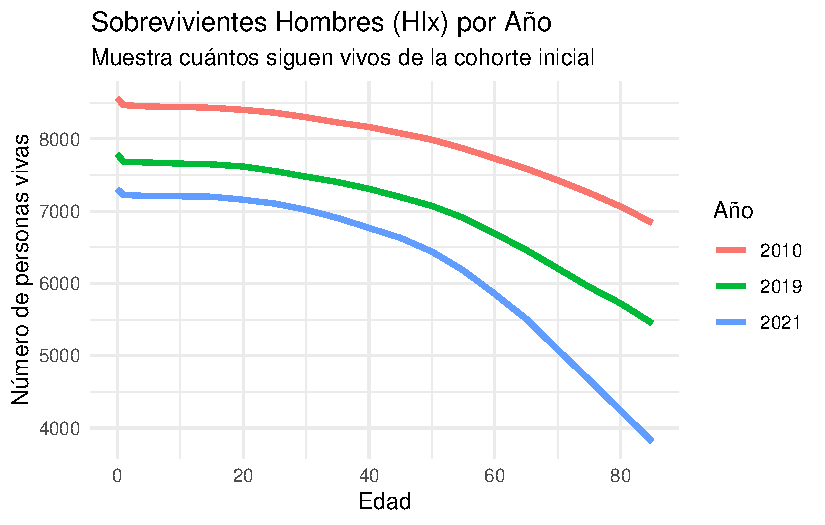
\includegraphics[keepaspectratio]{Informe_files/figure-pdf/unnamed-chunk-8-1.pdf}}

\pandocbounded{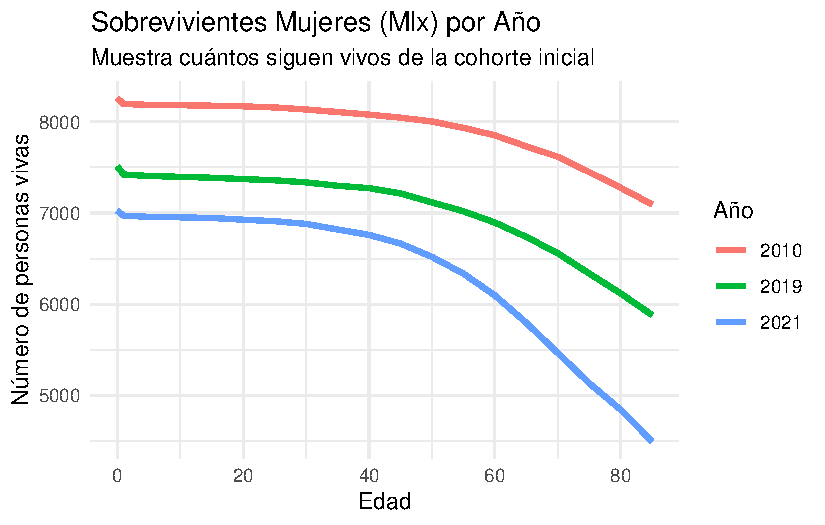
\includegraphics[keepaspectratio]{Informe_files/figure-pdf/unnamed-chunk-8-2.pdf}}

\pandocbounded{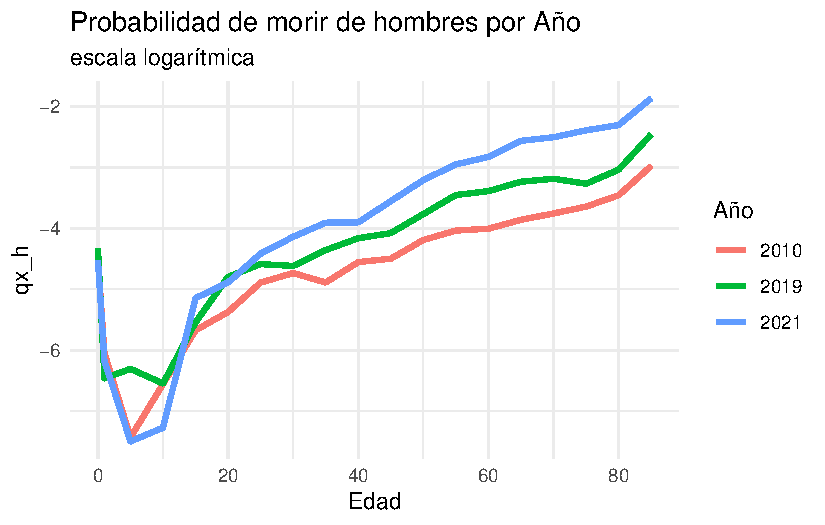
\includegraphics[keepaspectratio]{Informe_files/figure-pdf/unnamed-chunk-8-3.pdf}}

\pandocbounded{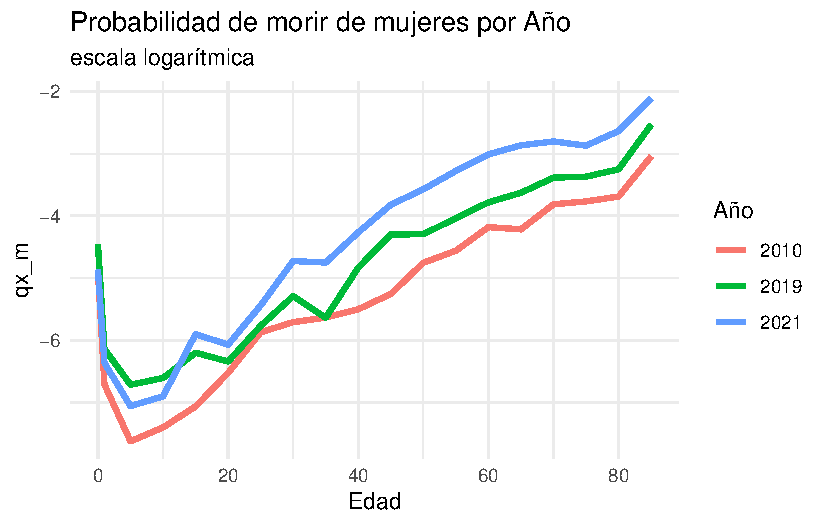
\includegraphics[keepaspectratio]{Informe_files/figure-pdf/unnamed-chunk-8-4.pdf}}

\section{Análisis}\label{anuxe1lisis}

Al comparar los años 2010, 2019 y 2021 se puede observar cómo cambió la
mortalidad en Campeche antes y durante la pandemia. El año 2010 sirve
como un punto de partida, mientras que 2019 permite ver la situación
antes de la COVID-19. Por otro lado, 2021 es importante porque refleja
el impacto que tuvo la pandemia en la mortalidad. En general, si entre
2010 y 2019 la esperanza de vida aumenta, esto puede interpretarse como
una mejora en las condiciones de supervivencia de la población. Es
decir, la población de Campeche habría tenido mejores condiciones de
salud o menor riesgo de morir en ciertos grupos de edad. Sin embargo, al
llegar a 2021, este comportamiento puede cambiar debido al aumento de
defunciones provocado por la COVID-19. Una de las partes más importantes
del análisis es comparar 2019 con 2021, porque 2019 representa un año
``normal'' antes de la pandemia, mientras que 2021 muestra un año
afectado por un evento sanitario fuerte. Si en 2021 aumenta la
probabilidad de morir qx, o disminuye la esperanza de vida e x, se puede
decir que la pandemia tuvo un efecto importante en la mortalidad del
estado. También hay que considerar algunas características de Campeche.
Es un estado con población relativamente pequeña y con baja densidad
poblacional, por lo que algunas personas pueden vivir lejos de los
principales servicios de salud. Esto puede influir en la atención médica
y en el comportamiento de la mortalidad. Además, Campeche ha tenido un
proceso de envejecimiento gradual, lo cual también puede aumentar la
mortalidad, ya que las personas adultas mayores tienen mayor riesgo de
morir. Por sexo, normalmente las mujeres tienen mayor esperanza de vida
que los hombres. Entonces, si en los resultados se observa que e x, de
las mujeres es mayor que el de los hombres, esto coincide con el
comportamiento esperado. En cambio, si en 2021 la esperanza de vida de
los hombres baja más, podría interpretarse como una mayor afectación
masculina durante la pandemia. En conclusión, los resultados muestran
que la mortalidad en Campeche no debe analizarse solo con los
indicadores y datos, sino también tomando en cuenta el contexto. Entre
2010 y 2019 se puede observar la evolución normal de la mortalidad, pero
en 2021 aparece el efecto de la COVID-19. Por eso, los cambios más
importantes de ese año pueden estar relacionados con la pandemia, el
envejecimiento de la población y las condiciones particulares del estado




\end{document}
